\documentclass[10pt,twocolumn,letterpaper]{article}
\usepackage[T1]{fontenc}
\usepackage[utf8]{inputenc}
\usepackage{lmodern}
\usepackage[hidelinks,pagebackref,breaklinks,colorlinks]{hyperref} % Hyperref package for url's and [hidelinks] option to remove collouring
\usepackage{bookmark}
\usepackage{graphicx}
\usepackage{amsmath}
\usepackage{amssymb}
\usepackage{booktabs}
\usepackage{caption}
\usepackage{subcaption}
\usepackage[capitalize]{cleveref}
\crefname{section}{Sec.}{Secs.}
\Crefname{section}{Section}{Sections}
\Crefname{table}{Table}{Tables}
\crefname{table}{Tab.}{Tabs.}

\begin{document}

\title{Object Detection and Spatial Relation}

\author{Saverio Sologni, Joginder Singh, Rocco De Ciantis}
\maketitle


\begin{abstract}
  \textit{This project aims to build a Computer Vision 
  system able to
  describe the spatial relationship between objects on the same image.
  The steps involved for fulfill this task are object detection and classification, 
  computation of the position and spatial reasoning.
  An instance segmentation network is used to detect the objects and distinguish 
  between different instances of the same class, which may happen in some images.
  This is needed for referring to the correct object when determine its position
  (center), which is obtained by computing the center of each previously 
  detected object.
  Each object is then compared with other objects in the image in order to determine
  how many objects are on left,right,top,down.
  }
\end{abstract}

\section{Introduction}
  The methodology we choose involves two main steps to produce our final output.
  A first offline pre-processing is done to all images in the dataset, in order to remove noise
  and provide all the informations needed to train and test the network for instance segmentation.
  Next we train and test the net on images, and do basic post-processing to get objects center.


\section{Dataset}
 The dataset used for this project is called Compositional Language and Elementary
   Visual Reasoning CLEVR .
  This dataset is designed with the explicit goal of enabling
  detailed analysis of visual reasoning. Its images depict
  simple 3D shapes like cubes, cylinders and spheres of different colors and sizes,
  arranged in different positions and in different numbers for each image.
  \\The dataset is a 70:15:15 dataset with 70000 images in the training set,
  15000 images in the validation set and 15000 in the test set.
  Objects depicted in the images are all been captured in gray background and
  they exhibit eight different colors:
   gray, blue, brown, yellow, red, green, purple, and cyan.
  \begin{figure}[t] %h sta per here (t per top e b per bottom)
  \centering
  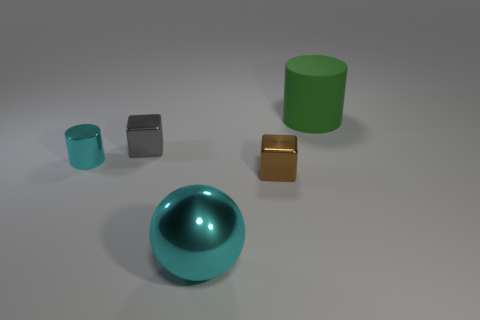
\includegraphics[scale=0.40]{images/datasetEx.png}
  \caption{\textit{A CLEVR dataset example image}}
  \label{datasetEx}
  \end{figure}
  Data as divided in two different conditions:
  \begin{itemize}
    \item \textbf{Condition A}
    \begin{itemize}
      \item Cubes are gray, blue, brown, or yellow
      \item Cylinders are red, green, purple, or cyan
      \item Spheres can have any color
    \end{itemize}
    \item  \textbf{Condition B}
    \begin{itemize}
      \item Cubes are red, green, purple, or cyan
      \item Cylinders are gray, blue, brown, or yellow
      \item Spheres can have any color
    \end{itemize}
  \end{itemize}
  The training set is made of images under \textbf{Condition A}, test set is made of
  images under \textbf{Condition B}.
  \\All of the objects are made of different materials that changes their brightness,
   showing light and objects reflections.
  The dataset includes also questions and answers in order to test
   various aspects of visual reasoning including
  attribute identification, counting, comparison, spatial relationships, and logical 
  operations.
  Each question in CLEVR is represented both in natural language and as a functional program.
  The functional program representation allows for precise determination of the
   reasoning skills required to answer each question.
  \\Nevertheless in this project \textit{only image data are used}, since our spatial reasoning task
  is limited to count the number of objects on left, right, above, below w.r.t. the current object.


\section{Preprocessing on Data}
  This offline preprocessing step is done in order to remove noise and prepare
  data to train the instance segmentation network.
  Extracted informations are a binary mask and a bounding box for 
  each object in each image, used as ground truth for training. 
  Since CLEVR do not provide such data, our goal is to retrieve them in 
  a fully automatic manner.\\
  \\ This includes three main steps:
  \begin{itemize}
    \item detect objects by their color;
    \item get a binary mask out of each selected object;
    \item get a bounding box out of each generated mask;
  \end{itemize}
  
  The first step is done by converting images in the HSV space,
   in which is simpler to retrieve pixel areas with
  specific colors; then, masks of pixels are obtained by selecting 
  pixels whose values assume a specific range in the color space.
  Masks are retrieved for every color in the dataset
   (red, green, purple, cyan, gray, blue, brown, or yellow).
  \\Since the dataset provides sets of generated 3D images, there is very little presence 
  of \textit{signal noise} (e.g. Gaussian), which is typical in images acquired by cameras. 
  Instead, images presents \textit{semantic noise} expressed as reflection of objects,
  light and background on metal surfaces, and as shadows on the background
  due to light illumination. This kind of noise makes the above mentioned step difficult
  without any sort of preprocessing:
  if an object is reflected on a surface, that portion of surface will also be
  detected when searching for objects of the same color of the reflected one; moreover,
  the reflection surfaces are themselves colored, hence the colors blends with each other
  generating a reflection that could be detected when searching for other colors, 
  as in Figure 2.
  \begin{figure}[h] %h sta per here (t per top e b per bottom)
    \centering
    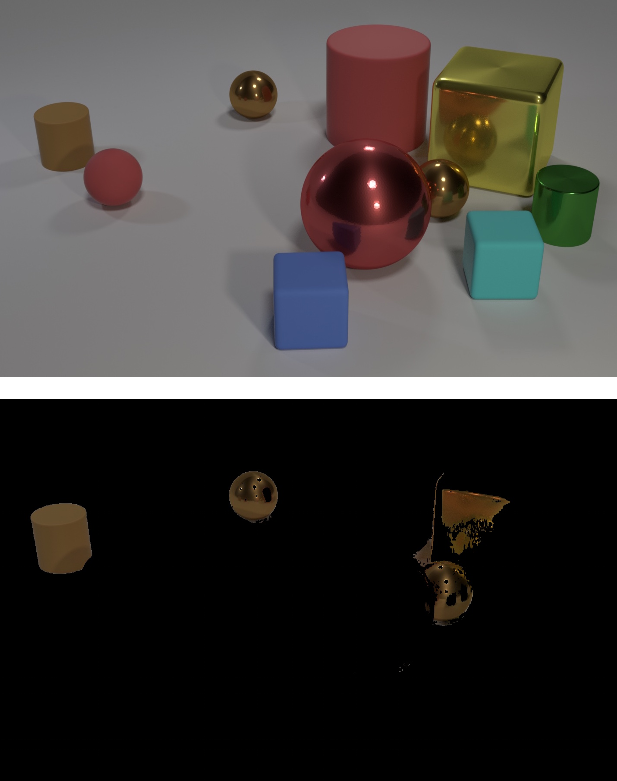
\includegraphics[scale=0.5]{images/noise_wrong.png}
    \caption{\textit{Brown and red spheres reflection on the
     yellow cube gets also detected when searching for brown objects}}
  \end{figure}
  \\Light reflection and shadows can also be sources of semantic noise: in Figure 2,
  bright areas on the metal spheres are not detected by the color mask,
  but is instead detected a small shadow area between red cylinder and the yellow cube.
  \\To cope with these problems a \textbf{bilateral filter} is applied to reduce reflection 
  while keeping sharp edges, and to smooth shadows;
  then background removal along with image labeling is done with \textbf{connected components}.
  Image labeling is done in order to distiguish between masks of the same color.
  \\Once obtained all the color masks, we need to associate them to the corresponing object
  for retrieve ground truth informations for training and testing:
   since the dataset provide it, the position (center) of each object is retrieved for
  associate it to the mask that has the center more close to it.
  Finally every mask get binarized and bounding boxes are retrieved out of each mask. 
  \begin{figure}[h] %h sta per here (t per top e b per bottom)
    \centering
    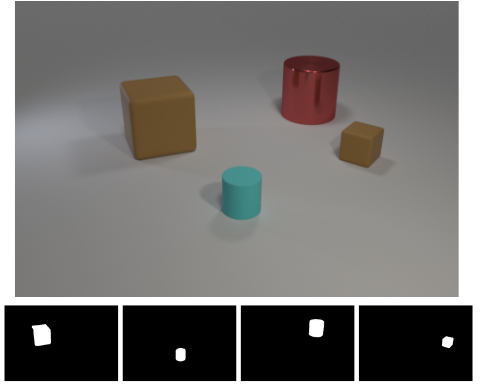
\includegraphics[scale=0.63]{images/preprocessing.png}
    \caption{\textit{One binarized mask for each object}}
  \end{figure}

\section{Network}
  Object detection and segmentation is done with a very known network: \textbf{MaskRCNN}.\\
  The model is implemented in \textit{PyTorch}, with ResNet-50 
  as backbone for feature extraction and classification, and a \textit{Region Proposal Network}
  (RPN) used for propose \textit{Region of Interests} (ROI) which will feed the rest 
  of the architecture in order to
   generate bounding boxes and class for detection, and masks for segmentation.
  \begin{figure}[h] %h sta per here (t per top e b per bottom)
    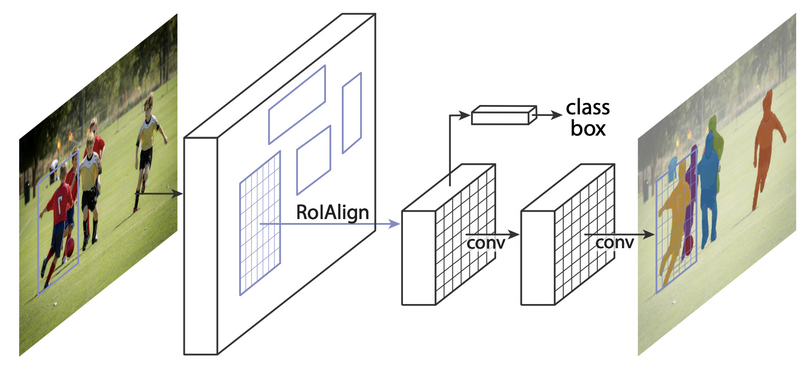
\includegraphics[scale=0.28]{images/mrcnn.png}
    \caption{\textit{MaskRCNN scheme }}
  \end{figure} \\
  Backbone weights are pre-trained with ImageNet data, while the rest is fine-tuned by
  training on CLEVR data.\\
  The network takes images of size 320$\times$480$\times$3 as input,
  and outputs a score for each object in the scene, the corresponing mask and bounding box.\\
  The network combine 5 losses in a single one:
  \begin{itemize}
    \item \textbf{Negative Log Likelyhood (NLL)}: used by the classifier. 
      This is a typical loss for multiclass classification tasks.
      The main objective is to find a set of model parameters $\theta$,
      that maximizes the likelyhood of observing data:
      by calling $\mathcal{D}$ our dataset, the goal is to find 
      the maximum likelyhood 
      \begin{center}
        $\mathbb{P}(\mathcal{D}|\theta) = \prod_{i=1}^{|\mathcal{D}|}\hat{y_i}$
      \end{center}
      where $\hat{y_i} = \sigma(f(\theta;x_i))$ is the output of the classifier
       $f(\theta;x_i)$ passed through a softmax function
       \begin{center}
        $\sigma(z_i) = \frac{\exp(z_i)}{\sum_{j=0}^{C-1}\exp(z_j)}$
       \end{center}
       used to feed the loss with probability scores.
       \\Applying logarithm and passing from a maximization to a minimization problem,
       the maximum likelyhood becomes:
       \begin{center}
        $\log(\mathbb{P}(\mathcal{D}|\theta)) = - \sum_{i=1}^{|\mathcal{D}|}\log(\hat{y_i})$
       \end{center}
    \item \textbf{SmoothL1}: used for \textit{bounding box generation} and \textit{RPN}. 
       It creates a criterion that uses a squared term if the absolute
       element-wise error of falls below 1, a L1 term otherwise.
       \newpage It is less sensitive to outliers than the \textit{Mean Squared Error (MSE)}.
       It is formulated as follows:
       \begin{center}
        $smoothL1loss(z_i)=\frac{1}{N} \sum_{i}z_i$
       \end{center}
       where
       \begin{center}
        $z_i = \begin{cases}
          \frac{1}{2}(y_i - \hat{y_i})^2 & \mbox{if} \,\,\, |y_i - \hat{y_i}| < 1\\
          |y_i - \hat{y_i}| -  \frac{1}{2} &  \mbox{otherwise}
        \end{cases}$
       \end{center} 

    \item \textbf{BinaryCrossEntropy}: used for \textit{objectness}
     (recognizing objects from background) and \textit{mask generation}.
     It is a measure of how close two distributions are, and 
     it is widely used to binary classification problems
     \begin{center}
      $ H = - \frac{1}{N} \sum_{i=1}^{N}(y_i \log(\hat{y_i}) + (1 - y_i)
      \log(1-\hat{y_i}))$
     \end{center}
  \end{itemize}

  The network combine this five losses in one single loss during training:
  \begin{center}
    $ loss = nll_{classifier} + smoothL1_{bb} + smoothL1_{rpn} +
    H_{objectness} + H_{mask}  $
  \end{center}



\section{Spatial Reasoning}
  The goal is to calculate the number of objects
  at the right, left, above, below for each object of 
  the image. 
  \\For each object detected by the network calculate the center ($x, y$),
  then take one object and compare its center with centers of other objects.
  \\Considering $\mathbb{O} $ as the set of objects in the image,
  for each $i \in \mathbb{O}$ fixed object,
    and for each $j \in \mathbb{O}\setminus\{i\} $ other object in the image:
  \begin{itemize}
    \item if $x_i < x_j $: $j$ is on the right of $i$ 
    \item if $x_i > x_j $: $j$ is on the left of $i$
    \item if $y_i < y_j $: $j$ is above $i$
    \item if $y_i > y_j $: $j$ is below $i$
  \end{itemize}

\section{Experiment}
\subsection*{Preprocessing}
  The offline preprocessing is applied to both train and test set,
  in order to obtain ground truth masks and bounding boxes for
  training and testing.
  \\Some adjustments are needed in the mask generation process:
   if two or more objects are close 
  enough such that one partially occlude the others, and if they are of the same
  materials, the resulting mask of each of these object will cover the same area
  and will have the same position of the other masks;
  this  happens because the objects are not far enough to generate two or more distinct 
  masks (distiguished with connected components) to associate to their relative objects, but there will a single mask to associate
  to all of these objects. So in this scenario, two objects with
  same color, same material and close to each other will have two identical masks covering
  the same pixel area corresponding to the area of both objects.

  \begin{figure}[h] %h sta per here (t per top e b per bottom)
    \centering
    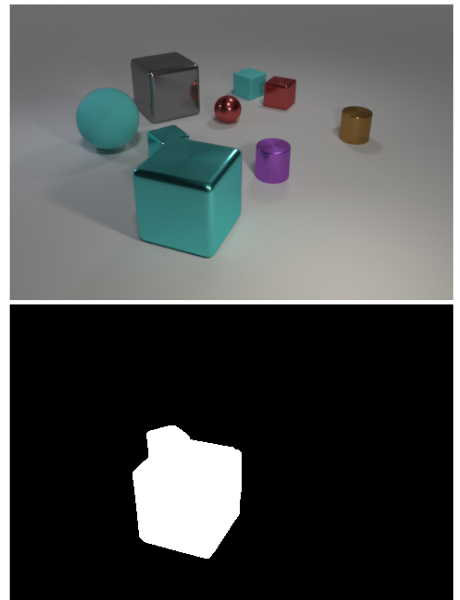
\includegraphics[scale=0.5]{images/bad_preprocessing.png}
    \caption{\textit{The generated mask is the same for both small and big
    metallic cyan cubes}}
  \end{figure}
  \newpage Since these are supposed to be ground truth data, they are not acceptable for training 
  and testing and for this reason all this kind of images are removed from the train 
  and test sets.
\subsection*{Training}
  We trained the network to detect and classify only 
  shapes of objects, so the classification task became a detection
  and segmentation of 3 shapes in total:
  cube, sphere, cylinder.  
  The network has been trained with \textbf{Stochastic Gradient Descent}
  (SGD) technique with a \textit{learning rate} of 0.005,
    \textit{momentum} of 0.9 and \textit{weight decay} of 0.005.

\subsection*{Testing}
  Since the dataset does not give crucial information to retrieve ground truth
  data of the test set, we opted to generate our test set with \textbf{Blender}, 
  the same software used to generate the entire CLEVR dataset; the generated set is then
  preprocessed to retrieve ground truth data. In order to properly test the network
  only the shape along with object centers are recovered; then both ground truth and 
  predicted data ( labels, bounding boxes, scores ) are sorted by the position of the
  corresponding object from left to righ, and finally metrics are calculated. 
  \\The metric used to test the net is the \textit{Mean Average Precision (MAP)}, a 
  standard metric used for object detection. MAP values for all
  \textbf{743} images of the test set
  were leveraged, obtaining the result of \textbf{0.8168} MAP.


\newpage
\section{Full Pipeline}
  Since the network classify only shapes, we retrieve the actual class of the objects by
  retrieving also the color for each detected shape:
  each predicted mask is overlapped with the original image,
  generating a new image with a mask that has the original color of the object.
  For each color (gray, blue, brown, yellow, red, green, purple, cyan)
   new masks are generated out of the overlapped image,
  and is taken the color that generate the mask that has maximum 
  \textit{Intersection Over Union} with the predicted one.
  \newline \newline So for each image, the MaskRCNN network detect shapes of objects,
  for each detected shape the actual class is retrieved by getting the color 
  that the object in question had; finally centers of predicted masks are calculated
  and compared in order to count the number of objects to the left, right, above , below 
  of each detected object in the image.
  

\end{document}